\documentclass[a4paper]{exam}
\usepackage[margin=1in]{geometry}
\usepackage{amsmath, amsfonts}
\usepackage{pythonhighlight}
\usepackage{graphicx} %package to manage images
% \graphicspath{ {./images/} }
\usepackage{hyperref}
\usepackage{tabularx}
\usepackage{colortbl}
\usepackage{algorithm}
\usepackage{algpseudocode}

\printanswers
\begin{document}
\begin{center}
{\Large \textbf{Spring 2024}}\vspace{1.0em}\\
{\Large \textbf{CS 412 (Algorithms: Design and Analysis)}}\vspace{1.0em}\\
{\Large \textbf{Weekly Challenge 04: }}\vspace{1.0em}\\
{\Large Announced: Friday, February 9, 2024.}\\
\vspace{.25em}
{\Large Deadline: Friday, February 16, 2024 (11:59 pm PKT).}\\ 
\vspace{.3em}
{\Large Total marks: 1.}
\vspace{.5em}\\
\end{center}
\textbf{Instructions}: Submit \textbf{individually} your solution as a PDF with the file name as your $studentID.pdf$; typeset in LaTeX. You must submit your solution on Canvas.

\centerline{\rule{.7\textwidth}{1pt}}
\begin{questions}
\question[1]
Imagine that you have a 2D grid where each cell contains a color value (see Figure \ref{figure1} for an example). Given a start location $(x, y)$, target color, and replacement color, design a recursive algorithm to fill closed regions with a specific color (replacement color). Clearly define a base criterion and analyze the worst-case time complexity of your proposed algorithm/approach. \\ 

Suppose that you have the following array:
\begin{figure}[h]
    \centering
    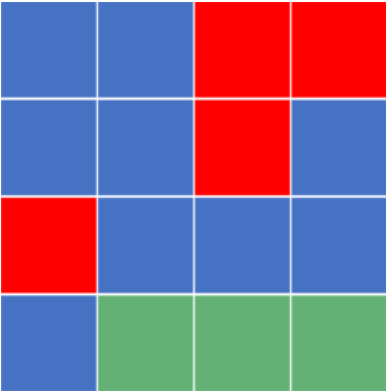
\includegraphics[scale=0.5]{image1.png}
    \caption{Before}
    \label{figure1}
\end{figure}

Now, we’re given a $start\_position = (0, 0)$ and $new\_color =$ orange. As we can see the color of cell $(0, 0)$ is blue. Therefore, we’ll recolor all its connected cells that have the same color to the $new\_color$:

\begin{figure}[h]
    \centering
    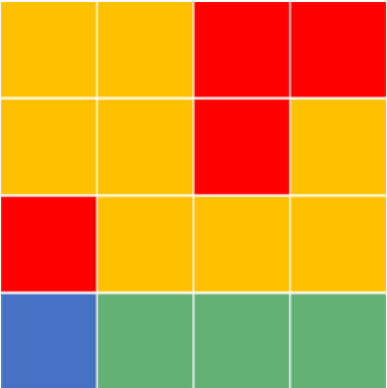
\includegraphics[scale=0.5]{image2.png}
    \caption{After}
\end{figure}

\textbf{Input}: start location (row, column), replacement color. \\
\textbf{Output}: replaces all adjacent cells with the target color with the replacement color. The target color is the original color of the starting location. \\
\textbf{Moves}: possible moves are up, down, left, right. In addition to up, down, left, and right, you can also add up-right, up-left, down-right, and down-left. \\
\textbf{Hint}: The algorithm might include recursive calls for each move. \\

% \begin{center}
%     \begin{table}[h!]
%         \centering
%         \scalebox{2}{
%         \begin{tabular}{|c|c|c|c|c|c|l|}
%             \hline
%             1 & 1 & 1 & 2 & 2 & 2 & \cellcolor{yellow!25}2 \\
%             \hline
%             1 & 1 & 2 & 2 & 2 & 2 & 2 \\
%             \hline
%             1 & 1 & 3 & 3 & 3 & 2 & 2 \\
%             \hline
%             2 & 1 & 3 & 3 & 3 & 2 & 2 \\
%             \hline
%             2 & 1 & 3 & 3 & 3 & 2 & 2 \\
%             \hline
%             2 & 1 & 3 & 3 & 3 & 2 & 2 \\
%             \hline
%             1 & 1 & 3 & 3 & 3 & 2 & 2 \\
%             \hline
%             1 & 1 & 3 & 3 & 3 & 2 & 2 \\
%             \hline
%         \end{tabular}}
%         \caption{The Results}
%         \label{fig1}
%     \end{table}
% \end{center}

\textbf{Note}: Figure \ref{figure1} is only an example, your algorithm should be valid for any number of colors and any arrangement of the colors.
% Add your solution here
\begin{solution}
        % \question Fill Region
        \begin{algorithm}[H]
        \caption{Fill Region}
        \begin{algorithmic}[1]
        \Function{FillRegion}{$\text{grid}, \text{start\_row}, \text{start\_col}, \text{target\_color}, \text{replacement\_color}$}
          \If{$\neg (0 \leq \text{start\_row} \text{ AND } \text{start\_row} < \text{len(grid)}) \text{ AND } (0 \leq \text{start\_col} \text{ AND start\_col}< \text{len(grid}[0]))$}
            \State \Return
          \EndIf
          \If{$\text{grid}[start\_row][start\_col] \neq \text{target\_color}$}
            \State \Return
          \EndIf
          \If{$\text{grid}[start\_row][start\_col] = \text{replacement\_color}$} \Comment{Already visited}
            \State \Return
          \EndIf
          \State $\text{grid}[start\_row][start\_col] \gets \text{replacement\_color}$ \Comment{Mark as visited}
          \State \Call{FillRegion}{$\text{grid}, \text{start\_row} + 1, \text{start\_col}, \text{target\_color}, \text{replacement\_color}$} \Comment{Explore adjacent cells}
          \State \Call{FillRegion}{$\text{grid}, \text{start\_row} - 1, \text{start\_col}, \text{target\_color}, \text{replacement\_color}$}
          \State \Call{FillRegion}{$\text{grid}, \text{start\_row}, \text{start\_col} + 1, \text{target\_color}, \text{replacement\_color}$}
          \State \Call{FillRegion}{$\text{grid}, \text{start\_row}, \text{start\_col} - 1, \text{target\_color}, \text{replacement\_color}$}
        \EndFunction
        \end{algorithmic}
        \end{algorithm}
    % \end{questions}
\end{solution}


\end{questions}


\end{document}
